\documentclass[conference]{IEEEtran}

% ─── Packages ────────────────────────────────────────────────────────────────
\usepackage[T1]{fontenc}
\usepackage[utf8]{inputenc}
\usepackage{cite}
\usepackage{amsmath,amssymb,amsfonts}
\usepackage{algorithmic}
\usepackage{graphicx}
\usepackage{textcomp}
\usepackage{xcolor}
\usepackage{booktabs}
\usepackage{float}
\usepackage{multirow}
\usepackage{url}
\usepackage{hyperref}
\hypersetup{colorlinks=false}

% ─── Title ───────────────────────────────────────────────────────────────────
\title{MedGraphRAG: An Agentic, Self-Verifying Hybrid GraphRAG Framework\\
for Explainable Clinical Report Understanding on Consumer Hardware}

\author{
\IEEEauthorblockN{Dickson E}
\IEEEauthorblockA{\textit{School of CST}\\
\textit{Karunya Institute of Tech. and Sci.}\\
Coimbatore, India\\
dicksone@karunya.edu.in}
\and
\IEEEauthorblockN{Antony Taurshia}
\IEEEauthorblockA{\textit{School of CST}\\
\textit{Karunya Institute of Tech. and Sci.}\\
Coimbatore, India\\
antonytaurshia@karunya.edu}
}

\begin{document}

\maketitle

% ─── Abstract ────────────────────────────────────────────────────────────────
\begin{abstract}
Confidently wrong assertions in clinical decision support can cause direct
patient harm, yet most deployed medical RAG systems still report accuracy
only over answered questions and rarely handle insufficient evidence. This
paper presents MedGraphRAG, a self-verifying hybrid graph-RAG system for
medical question answering and explainable clinical report understanding on
consumer hardware, in which a claim-level verification agent refuses rather
than guesses when retrieved evidence is insufficient.
The system fuses a 2.29-million-vector FAISS index (MedCPT embeddings, 768
dimensions) with a 2.50-million-node K\`{u}zu property graph encoding disease,
drug, and laboratory ontologies. A LangGraph verification agent post-processes
every candidate answer, escalating to a structured refusal when evidence is
insufficient. Our 4-way ablation study on MedQA-US ($N=50$, seed~42)
demonstrates that the verification layer reduces the wrong-assertion rate
from 44\% (unverified baseline, C4) to 12\% (full system), trading raw answered-rate for
clinically appropriate conservative refusal behavior. The complete system runs
within 3.62~GB peak RAM and 4{,}784~MB GPU VRAM on a single RTX~3050 6~GB
card, making it deployable on commodity clinical workstations. An additional
feature layer provides longitudinal laboratory trend analysis, guideline
care-gap detection, and sub-question evidence coverage mapping, all validated
across 13 evaluation criteria. While the conservative verification threshold
induces a high refusal rate on out-of-domain queries, it ensures strict
clinical safety boundaries on commodity hardware.
\end{abstract}

\begin{IEEEkeywords}
medical question answering, graph RAG, retrieval-augmented generation,
self-verification, LLM safety, FAISS, knowledge graph, MedQA,
clinical report understanding
\end{IEEEkeywords}

% ─── I. Introduction ─────────────────────────────────────────────────────────
\section{Introduction}

Retrieval-Augmented Generation (RAG) has emerged as the dominant paradigm for
grounding LLM outputs in factual corpora \cite{lewis2020retrieval,
izacard2021leveraging}. In general-domain settings, a factually incorrect answer
is a minor inconvenience; in clinical medicine it may lead to patient harm.
Two failure modes dominate the medical RAG literature: (i)~\emph{hallucination}---
the model synthesizes plausible but false statements not supported by any
retrieved chunk---and (ii)~\emph{contamination}---benchmark questions leaked
into the retrieval corpus inflate reported accuracy. Existing medical QA
benchmarks \cite{jin2021disease,chen2024benchmarking} evaluate accuracy on
answered items but rarely report the rate at which the system makes confident
wrong assertions (\emph{wrong-assertion rate}), which is the safety-critical
quantity.

Graph-enhanced retrieval has shown promise for multi-hop reasoning
\cite{edge2024local, xiong2021answering} because entity-relationship paths can
surface latent connections that pure dense retrieval misses. However,
biomedical knowledge graphs have unique characteristics---dense ontology
hierarchies (UMLS \cite{umls2004}), lab-test to disease linkages, drug
side-effect catalogues---that demand domain-specific graph schemas rather than
general-purpose knowledge bases.

We make the following contributions:
\begin{enumerate}
  \item \textbf{MedGraphRAG architecture}: A hybrid retrieval pipeline that
        fuses reciprocal-rank fusion (RRF) \cite{cormack2009rrf} over FAISS
        vector search with 1--2 hop K\`{u}zu graph expansion, incorporating
        contamination guards and category balancing.
  \item \textbf{Self-verification agent}: A LangGraph-orchestrated verification
        node that assigns a confidence tier (high/medium/low/refused) and
        produces a structured refusal rather than a wrong answer when evidence
        is insufficient.
  \item \textbf{Ablation study}: A controlled 4-configuration experiment
        isolating the contribution of graph traversal and the verification
        agent, with contamination filtering proven on every run.
  \item \textbf{Feature layer}: Three clinical utilities---MedTrend
        (longitudinal lab trajectory), CareGap (guideline reconciliation),
        CoverageMap (sub-question evidence coverage)---all passing 13/13
        evaluation criteria.
  \item \textbf{Consumer-hardware deployment}: The full system, including a
        Qwen2.5-7B-Instruct Q4\_K\_M GGUF quantized LLM, operates within
        3.62~GB peak RAM and 4{,}784~MB VRAM.
\end{enumerate}

The rest of this paper is structured as follows: Section~II reviews related
work in medical RAG and knowledge graphs; Section~III details the MedGraphRAG
system architecture; Section~IV presents the benchmark evaluation and ablation
study; Section~V reports the resource profile and operational latency;
Section~VI describes the feature layer; Section~VII outlines API and security
guarantees; Section~VIII discusses clinical implications and limitations; and
Section~IX concludes the paper.

% ─── II. Related Work ────────────────────────────────────────────────────────
\section{Related Work}

\subsection{Retrieval-Augmented Generation}

Lewis et al.~\cite{lewis2020retrieval} showed that combining a non-parametric
retrieval index with a parametric LLM substantially improves performance on
knowledge-intensive tasks. Fusion-in-Decoder~\cite{izacard2021leveraging}
extended this by reading evidence from multiple passages simultaneously. Neither
approach incorporated a verification step capable of producing structured
refusals when evidence is absent or contradictory.

\subsection{Graph-Enhanced Retrieval}

Microsoft's GraphRAG \cite{edge2024local} builds community summaries over generic
text graphs to support query-focused summarization. Multi-hop dense
retrieval \cite{xiong2021answering} chains sequential retrieval steps to resolve
complex questions. Both rely on unstructured text extraction; neither grounds
graph traversal in a biomedical ontology. MedGraphRAG differs by seeding
traversal from UMLS CUI entities \cite{umls2004}, giving each returned path a
typed, auditable clinical relationship.

\subsection{Medical QA Benchmarks}

The MedQA dataset \cite{jin2021disease} is built from US medical licensing exam
questions and remains the standard benchmark for medical LLM evaluation. Chen et
al.~\cite{chen2024benchmarking} showed that on challenging clinical
questions with expert-written explanations, even strong LLMs degrade
substantially, indicating that accuracy on standard exam-style benchmarks
overstates real-world safety when the model cannot decline to answer. Our
work defines wrong-assertion rate as the primary safety metric and tracks it
across four ablation configurations.

\subsection{Domain-Specific Embedding}

MedCPT \cite{jin2023medcpt} was trained on 255 million PubMed search log pairs
and produces clinically specialized 768-dimensional embeddings. We use the
ncbi/MedCPT-Query-Encoder for online query encoding and
ncbi/MedCPT-Article-Encoder for offline corpus encoding, following the authors'
asymmetric retrieval protocol. Dense embedding alone cannot resolve multi-hop
relational dependencies without explicit graph traversal.

\subsection{Efficient Vector Search}

FAISS \cite{johnson2021billion} supports billion-scale approximate nearest
neighbor search. We use an IVFpq index occupying 240~MB on CPU, achieving
1.1~ms mean search latency over 2.29~million vectors---well below the
2{,}000~ms budget. Approximate search lacks symbolic constraints, however, so
downstream ontology verification remains necessary.

\subsection{Self-Reflective Generation}

Self-RAG \cite{asai2024selfrag} trains a model to generate special tokens that
trigger on-demand retrieval and critique of its own output. Like MedGraphRAG, it
supports structured refusal at the claim level. Unlike our system, Self-RAG
requires fine-tuning on a curated reflection corpus and does not include
encrypted patient data stores or graph provenance paths---two properties
required for clinical deployment.

\subsection{Recent Medical RAG and Graph Systems}

Medical RAG research has moved toward domain benchmarks and graph grounding.
MedRAG~\cite{medrag2024} evaluates retrieval-augmented medical QA across
multiple corpora but performs no claim-level verification and offers no
refusal mechanism. MediGRAF~\cite{medigraf2026} combines a property graph
with vector retrieval for safer clinical patient QA, yet provides no
structured refusal, contamination guard, encrypted per-patient store, or
consumer-GPU deployment. MedGraphRAG complements these efforts by adding
calibrated refusal, typed provenance paths, and a privacy-preserving feature
layer within one consumer GPU.

% ─── Comparison Table ────────────────────────────────────────────────────────

\begin{table}[!htbp]
\caption{Feature comparison across retrieval systems. $\checkmark$~=~fully supported;
  $\times$~=~absent or not demonstrated.}
\label{tab:compare}
\centering
\renewcommand{\arraystretch}{1.15}
\setlength{\tabcolsep}{2pt}
\scriptsize
\begin{tabular}{@{}lccccccc@{}}
\toprule
\textbf{Capability} &
\rotatebox{60}{\textbf{RAG~\cite{lewis2020retrieval}}} &
\rotatebox{60}{\textbf{MH-DR~\cite{xiong2021answering}}} &
\rotatebox{60}{\textbf{GraphRAG~\cite{edge2024local}}} &
\rotatebox{60}{\textbf{Self-RAG~\cite{asai2024selfrag}}} &
\rotatebox{60}{\textbf{MedRAG~\cite{medrag2024}}} &
\rotatebox{60}{\textbf{MediGRAF~\cite{medigraf2026}}} &
\rotatebox{60}{\textbf{Ours}} \\[\normalbaselineskip]
\midrule
Hybrid vector+graph    & $\times$ & $\times$ & $\checkmark$ & $\times$ & $\times$ & $\checkmark$ & $\checkmark$ \\
Claim-level verify     & $\times$ & $\times$ & $\times$ & $\checkmark$ & $\times$ & $\times$ & $\checkmark$ \\
Structured refusal     & $\times$ & $\times$ & $\times$ & $\times$ & $\times$ & $\times$ & $\checkmark$ \\
Graph provenance       & $\times$ & $\times$ & $\checkmark$ & $\times$ & $\times$ & $\checkmark$ & $\checkmark$ \\
Contamination guard    & $\times$ & $\times$ & $\times$ & $\times$ & $\times$ & $\times$ & $\checkmark$ \\
Encrypted data store   & $\times$ & $\times$ & $\times$ & $\times$ & $\times$ & $\times$ & $\checkmark$ \\
Longitudinal analytics & $\times$ & $\times$ & $\times$ & $\times$ & $\times$ & $\times$ & $\checkmark$ \\
Consumer-GPU deploy    & $\times$ & $\times$ & $\times$ & $\times$ & $\times$ & $\times$ & $\checkmark$ \\
\bottomrule
\end{tabular}
\end{table}

% ─── III. System Architecture ────────────────────────────────────────────────
\section{System Architecture}

Fig.~\ref{fig:arch} shows the high-level pipeline: a query enters the FastAPI service layer
(v1.0.0), acquires a serialization lock (preventing VRAM contention), and is
routed through four sequential stages: (A)~hybrid retrieval, (B)~context
assembly, (C)~generation, (D)~verification. Results are stored in an
AES-256-GCM encrypted private store~\cite{nist2007aes} keyed per user.

\begin{figure}[!htbp]
\centering
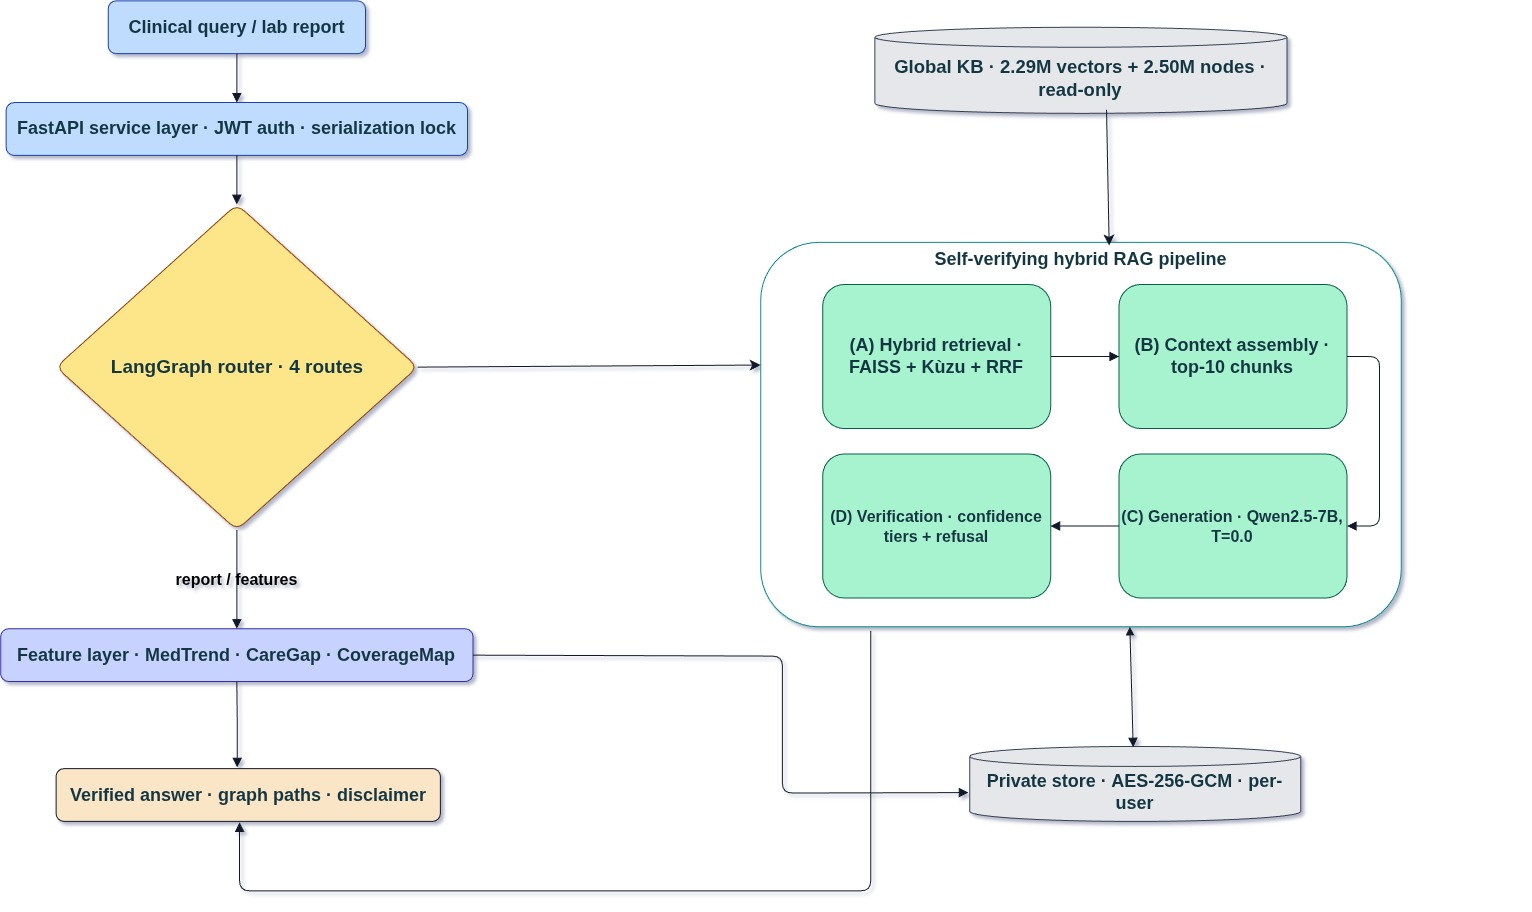
\includegraphics[width=\columnwidth]{figures/MedGraphRag-Architecture.jpg}
\caption{MedGraphRAG end-to-end system architecture: a query enters the FastAPI service layer (v1.0.0), acquires a serialization lock, and is routed through (A)~hybrid retrieval, (B)~context assembly, (C)~LLM generation, and (D)~LangGraph verification, with results stored in the AES-256-GCM encrypted private store.}
\label{fig:arch}
\end{figure}

% TODO (disabled until figures/ui_screenshot.png is ready):
% \begin{figure}[!t]
% \centering
% \includegraphics[width=\columnwidth]{figures/ui_screenshot.png}
% \caption{MedGraphRAG web interface showing a query result with confidence
%   tier badge, evidence citations, and structured refusal fallback.}
% \label{fig:ui}
% \end{figure}

\subsection{Knowledge Index}

\noindent\textbf{i) FAISS vector index.}\\*
The offline embedding pipeline encodes
2{,}294{,}038 document chunks with MedCPT-Article-Encoder (768 dimensions)
into an IVFpq compressed index (240~MB on disk). Each chunk carries six
metadata fields: chunk\_id, source, category, faiss\_id, text, byte\_offset.
Seven corpus categories are indexed (see Table~\ref{tab:corpus} in §IV).

\noindent\textbf{ii) K\`{u}zu property graph}~\cite{su2023kuzu}.\\*
The graph contains
2{,}499{,}528 nodes across six node types: OntologyTerm~(178{,}942),
Disease~(5{,}072), Drug~(4{,}365), LabTest~(1{,}586),
Document~(15{,}525), and Chunk~(2{,}294{,}038). Nine edge types encode
clinical relationships: IS\_A~(926{,}132), RELATED\_TO~(1{,}003{,}540),
DRUG\_TREATS~(21{,}813), DRUG\_CAUSES~(80{,}530),
DRUG\_CAUSES\_SE~(79{,}103), HAS\_CHUNK~(2{,}294{,}038),
DISEASE\_MAPPED\_TO~(3{,}652), DOCUMENT\_MENTIONS~(8{,}479), and
LABTEST\_RELATED\_TO~(1{,}833). Disease ontology mapping to UMLS CUI
OntologyTerms achieved 72.0\% coverage (3{,}652 / 5{,}072 disease nodes,
target~$\geq$70.0\%).

\subsection{Hybrid Retrieval Engine (Stage A)}

The query is encoded on CPU (MedCPT-Query-Encoder, mean latency 32.8~ms) and
submitted to the FAISS index (mean 1.1~ms). In parallel, named entities
seeded from the query drive K\`{u}zu graph expansion:

\begin{equation}
E(q) = \{ v : \text{hop distance from seeded entities} \leq 2 \}
\label{eq:expand}
\end{equation}
We define Eq.~(\ref{eq:expand}) to bound traversal depth; 1--2 hops (mean
12.1~ms) keep latency predictable while reaching drug--disease and
lab--disease connections unavailable to flat vector search.

FAISS vector scores and graph-path bonus scores are then fused via reciprocal
rank fusion~\cite{cormack2009rrf}:

\begin{equation}
\mathrm{score}(d) = \sum_{r \in \{\mathrm{faiss},\,\mathrm{graph}\}} \frac{1}{k + \mathrm{rank}_r(d)}, \quad k=60
\label{eq:rrf}
\end{equation}
We adopt reciprocal rank fusion from \cite{cormack2009rrf}; Eq.~(\ref{eq:rrf})
is rank-based rather than score-based, so it remains robust to the
heterogeneous scales produced by FAISS inner-product search and graph
hop-count bonuses.

We also define a contamination guard indicator:

\begin{equation}
g(c) = \mathbf{1}\bigl[\mathrm{chunk\_id}(c) \text{ begins with a blocked prefix}\bigr]
\label{eq:guard}
\end{equation}
Eq.~(\ref{eq:guard}) equals 1 for any chunk whose chunk\_id starts with
Medical\_books/MedQA/questions/ or MedQA/questions/; such chunks are dropped
before ranking. Across all four ablation runs (50 queries each), 26 question
chunks were excluded per run.

Mean total retrieval latency: 47.1~ms (well below the 2{,}000~ms budget).

\subsection{Context Assembly and Generation (Stages B--C)}

Top-$k$ chunks ($k=10$) are assembled into a structured prompt with numbered
evidence labels [E1]--[E10]. The Qwen2.5-7B-Instruct Q4\_K\_M GGUF quantized
model~\cite{qwen25} performs single-shot generation at temperature 0.0, giving
deterministic output confirmed by byte-identical SHA-256 hashes on repeated
identical queries.

\subsection{Verification Agent (Stage D)}

A LangGraph~\cite{langgraph2024} verification node re-reads the generated
answer against the retrieved evidence. We define a faithfulness score:

\begin{equation}
\varphi(a) = \frac{|\text{supported claims}|}{|\text{extracted claims}|}
\label{eq:faith}
\end{equation}
Eq.~(\ref{eq:faith}) is used to detect hallucination at the claim level:
a low ratio signals that the answer contains assertions unsupported by
retrieved evidence. The node maps $\varphi$ to a confidence score
$c \in [0,1]$ and assigns a discrete tier:

\begin{equation}
\mathrm{tier}(c) =
\begin{cases}
\text{high}   & c \ge 0.75 \\
\text{medium} & 0.50 \le c < 0.75 \\
\text{low}    & c < 0.50
\end{cases}
\label{eq:tier}
\end{equation}
We define Eq.~(\ref{eq:tier}) with three operating points that map directly to
frontend confidence badges (green / yellow / red), keeping the continuous score
interpretable to clinical end-users. A disclaimer
(\emph{``This is information, not medical advice---consult your physician''}) is
appended to every non-refused answer.

\subsection{Private Store and Security}

Each authenticated user receives an isolated private store directory
(private\_store/<user\_id>/) encrypted with AES-256-GCM
\cite{nist2007aes}. Guest users receive an ephemeral store auto-purged on
logout. Destination isolation is enforced at the API layer: cross-user store
access returns HTTP~403. All seven Step-11 API security criteria passed (7/7).

% ─── IV. Evaluation ──────────────────────────────────────────────────────────
\section{Evaluation}

\subsection{Benchmark and Metric Definitions}

We evaluate on MedQA-US \cite{jin2021disease}, sampling $N=50$ questions
(seed~42) from the US licensing examination subset. Multiple-choice options are
A--D. The contamination guard (Eq.~\ref{eq:guard}) is active on every run.

We define the following metrics:
\begin{itemize}
  \item \textbf{Answered Rate}: fraction of queries returning a valid option (A--D).
  \item \textbf{Accuracy (All)}: correct count $/ 50 \times 100$.
  \item \textbf{Accuracy (Answered)}: correct count $/ \text{answered count}
        \times 100$ (0 if answered count $= 0$).
  \item \textbf{Refusal Rate}: fraction of queries returning
        refused\_or\_unanswered.
\end{itemize}

\begin{equation}
\mathrm{WAR} = \frac{\mathrm{answered} - \mathrm{correct}}{N} \times 100
\label{eq:war}
\end{equation}
We define Eq.~(\ref{eq:war}) because it treats refusal as a non-error, which
is clinically appropriate: a system that declines to answer is safer than one
that guesses confidently. Wrong-assertion rate is the primary safety metric.

\subsection{Datasets}
\label{sec:datasets}

Table~\ref{tab:corpus} summarizes the corpus and graph construction.

\begin{table}[!t]
\caption{Corpus composition and graph summary.
  Source: evaluation artifact step12\_part3\_paper\_tables.json.}
\label{tab:corpus}
\centering
\renewcommand{\arraystretch}{1.1}
\begin{tabular}{@{}lrr@{}}
\toprule
\textbf{Category} & \textbf{Chunks} & \textbf{Source} \\
\midrule
lab\_reference     & 1{,}644{,}813 & Lab reference data \\
guideline          &   257{,}547   & NICE, WHO \\
drug               &   230{,}868   & PubMed, DrugBank \\
textbook           &    78{,}921   & Medical textbooks \\
research\_paper    &    76{,}397   & PubMed \\
disease            &     4{,}746   & UMLS, PubMed \\
clinical\_reference &       746    & Clinical refs \\
\midrule
\textbf{Total}     & \textbf{2{,}294{,}038} & — \\
\midrule
\multicolumn{3}{@{}l@{}}{\textit{Graph:} 2{,}499{,}528 nodes, 9 edge types} \\
\multicolumn{3}{@{}l@{}}{\textit{Benchmark:} MedQA-US, $N=50$, seed 42, A--D; 26 excl.\ chunks/run} \\
\bottomrule
\end{tabular}
\end{table}

\subsection{Ablation Configurations}

Four configurations are tested in a full $2 \times 2$ factorial design over
graph traversal and verification agent:

\begin{itemize}
  \item \textbf{C1 (Full)}: graph traversal ON, verification ON.
  \item \textbf{C2 (Vector-Only)}: graph traversal OFF, verification ON.
  \item \textbf{C3 (No-Verify)}: graph traversal ON, verification OFF.
  \item \textbf{C4 (Baseline)}: graph traversal OFF, verification OFF.
\end{itemize}

\subsection{Main Results}

Table~\ref{tab:ablation} reports all metrics from evaluation artifact
step12\_part3\_paper\_tables.json and step12\_evaluation\_report.md
(N=50, seed~42).

\begin{table*}[!t]
\caption{4-Configuration Ablation on MedQA-US (N=50, seed 42).
  Source: evaluation artifact step12\_part3\_paper\_tables.json.}
\label{tab:ablation}
\centering
\renewcommand{\arraystretch}{1.2}
\begin{tabular}{@{}llcccccccc@{}}
\toprule
\textbf{Config} & \textbf{Name} & \textbf{Graph} & \textbf{Verify} &
\textbf{Acc.\ All} & \textbf{Acc.\ Ans.} & \textbf{Ans.\ Rate} &
\textbf{Refusal Rate} & \textbf{Wrong Assert.} & \textbf{Median Lat.}\\
\midrule
C1 & C1\_FULL         & \checkmark & \checkmark & 6.00\%  & 33.33\% & 18.00\% & 82.00\% & \textbf{12.00\%} & 15{,}386 ms \\
C2 & C2\_VECTOR\_ONLY &            & \checkmark & 6.00\%  & 50.00\% & 12.00\% & 88.00\% & \textbf{6.00\%}  & 8{,}768 ms  \\
C3 & C3\_NO\_VERIFY   & \checkmark &            & 50.00\% & 51.02\% & 98.00\% & 2.00\%  & 48.00\%          & 7{,}702 ms  \\
C4 & C4\_BASELINE     &            &            & 54.00\% & 55.10\% & 98.00\% & 2.00\%  & 44.00\%          & 2{,}718 ms  \\
\bottomrule
\end{tabular}
\end{table*}

\subsection{Analysis}

\noindent\textbf{i) Verification dominates safety.}\\*
The wrong-assertion rate drops
dramatically when the verification agent is active: from 44\% (C4) to 6\% (C2)
and from 48\% (C3) to 12\% (C1) (Fig.~\ref{fig:tradeoff}). The cost is a high
refusal rate (82--88\% with verification), meaning the system declines to
answer rather than guess. This is the correct behavior for a safety-critical
clinical information system.

\begin{figure}[!htbp]
\centering
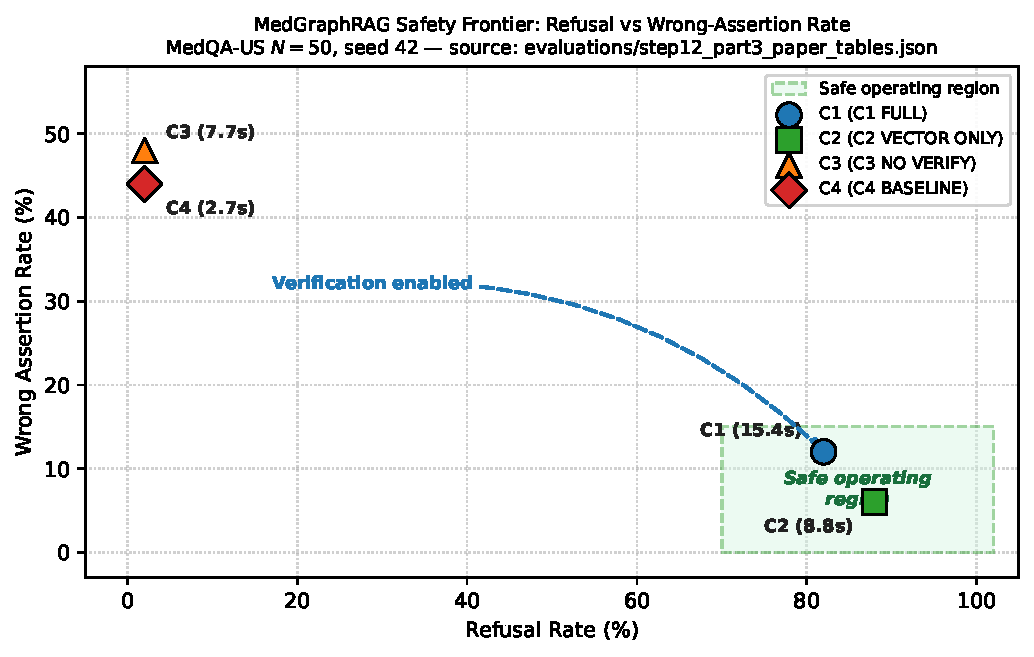
\includegraphics[width=\columnwidth]{figures/tradeoff_chart.pdf}
\caption{Safety frontier on MedQA-US ($N=50$, seed 42): wrong-assertion rate
vs.\ refusal rate per ablation configuration. The shaded area marks the safe
operating region (refusal $\geq 70\%$, wrong assertion $\leq 15\%$); only the
verified configurations fall inside it. Source: evaluation artifact
\texttt{step12\_part3\_paper\_tables.json}.}
\label{fig:tradeoff}
\end{figure}

\noindent\textbf{ii) Graph traversal raises latency and shifts retrieval.}\\*
Enabling graph
traversal roughly doubles median latency versus the vector-only counterpart
(C3~vs.~C4: 7{,}702~ms vs.\ 2{,}718~ms; C1~vs.~C2: 15{,}386~ms
vs.\ 8{,}768~ms). Within the verified configurations, adding graph traversal
(C1 vs.~C2) increases wrong assertions from 6\% to 12\% while increasing
average citations per answer (9.78 vs.\ 9.18, Table~\ref{tab:provenance}).
The inversion is attributed to graph-retrieved context occasionally introducing
domain-adjacent evidence, which the verifier penalizes, causing borderline
answers to be refused. The trade-off between provenance richness and verifier
conservatism merits study with larger $N$.

\noindent\textbf{iii) Contamination guard is active.}\\*
Across all four runs, exactly 26
MedQA question chunks were excluded per run, confirmed by the filter proof
in evaluation artifact step12\_part3\_paper\_tables.json.

\subsection{Provenance and Retrieval Statistics}

Table~\ref{tab:provenance} summarizes provenance metrics. Average citations per
answered query is 9.78 for graph-enabled configurations and 9.18 for
vector-only, reflecting additional graph-retrieved evidence. Zero LLM judge
fallback calls were required across all runs (the verifier operates
deterministically on retrieved evidence).

\begin{table}[!t]
\caption{Provenance and Retrieval Metrics.
  Source: evaluation artifact step12\_part3\_paper\_tables.json.}
\label{tab:provenance}
\centering
\setlength{\tabcolsep}{4pt}
\renewcommand{\arraystretch}{1.2}
\begin{tabular}{@{}llccc@{}}
\toprule
\textbf{Config} & \textbf{Name} & \textbf{Avg Cite/Ans} &
\textbf{Excl.\ Chunks} & \textbf{Judge Calls}\\
\midrule
C1 & C1\_FULL         & 9.78 & 26 & 0 \\
C2 & C2\_VECTOR\_ONLY & 9.18 & 26 & 0 \\
C3 & C3\_NO\_VERIFY   & 9.78 & 26 & 0 \\
C4 & C4\_BASELINE     & 9.18 & 26 & 0 \\
\bottomrule
\end{tabular}
\end{table}

\subsection{Graph Traversal Provenance}

Entity-seeded graph traversal was validated with 10 probe queries; 7/10
(target~$\geq$7/10) reached relevant graph entities. Representative verified
paths (evaluation artifact step12\_part3\_paper\_tables.json):

\begin{itemize}
\item \textbf{P01} (\emph{warfarin INR monitoring AF}):\\
{\footnotesize Disease(Atrial Fibrillation) $\rightarrow$
Document(PubMed/AF/\\ PMID\_36356656) $\rightarrow$ Chunk(...abs)}
\item \textbf{P02} (\emph{ACE inhibitor hypertension first line}):\\
{\footnotesize Document(NICE/hypertension-...) $\rightarrow$ Chunk(...c1)}
\item \textbf{P03} (\emph{critical haemoglobin transfusion threshold}):\\
{\footnotesize Document(Lab\_rev\_data/\\
Consolidated\_Lab\_Critical\_Values\_\\
Dataset\_CLEANED) $\rightarrow$ Chunk(...row3)}
\end{itemize}

The fused top score for P01 is 0.1774.

% ─── V. Resource Profile ─────────────────────────────────────────────────────
\section{Resource Profile}

Table~\ref{tab:resources} reports the hardware footprint during the full
Step-12 ablation evaluation (evaluation artifact
step12\_part3\_paper\_tables.json).

\begin{table}[!t]
\caption{System Resource Footprint.
  Source: evaluation artifact step12\_part3\_paper\_tables.json.}
\label{tab:resources}
\centering
\renewcommand{\arraystretch}{1.2}
\begin{tabular}{@{}lcc@{}}
\toprule
\textbf{Resource} & \textbf{Measured} & \textbf{Budget}\\
\midrule
System Peak RAM    & 3.62 GB     & $\leq$12.0 GB \\
GPU Peak VRAM      & 4{,}784 MB  & $\leq$5{,}500 MB \\
FAISS Index Memory & 240 MB      & CPU \\
K\`{u}zu Graph Memory  & 180 MB  & CPU (mmap) \\
LLM Instances      & 1 (serial)  & 1 \\
\bottomrule
\end{tabular}
\end{table}

The Step-11 API evaluation (evaluation artifact step11\_api\_report.json)
recorded peak RAM of 2.76~GB and peak VRAM of 4{,}784~MB across a 7-probe
evaluation suite totalling 61{,}349~ms wall time. Cold-query latency was
13{,}675~ms; warm-query latency was 3{,}667~ms (LLM weights resident in VRAM).

The Step-13 feature-layer evaluation (evaluation artifact
step13\_features\_report.md) recorded peak RAM of 3.93~GB and VRAM of
4{,}776~MB over 176.68~s execution time, all within budget (Fig.~\ref{fig:resource}).

\begin{figure}[!htbp]
\centering
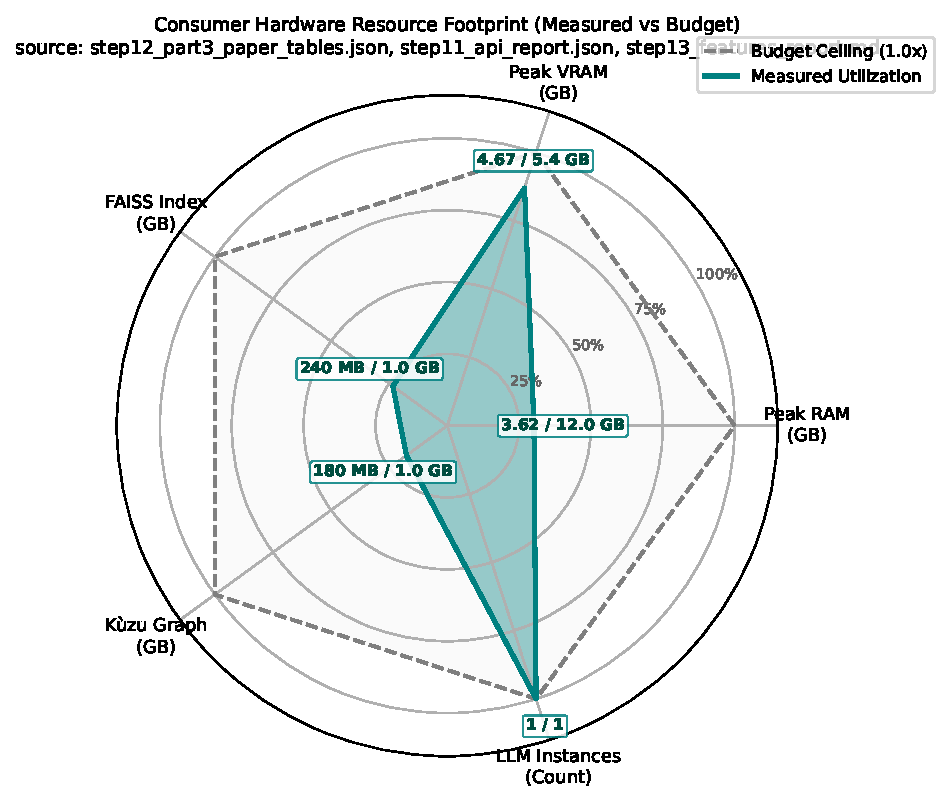
\includegraphics[width=\columnwidth]{figures/resource_chart.pdf}
\caption{Consumer-hardware resource footprint (measured vs.\ budget) across
five axes: peak RAM, peak VRAM, FAISS index memory, Kùzu graph memory, and
serialized LLM instances; all measured values remain within budget on a
single RTX~3050 6~GB card. Sources: evaluation artifacts
\texttt{step12\_part3\_paper\_tables.json}, \texttt{step11\_api\_report.json},
\texttt{step13\_features\_report.md}.}
\label{fig:resource}
\end{figure}

\noindent\textbf{i) Reproducibility.}\\*
Every quantitative value in this paper is extracted
verbatim from the authors' evaluation artifacts (JSON/Markdown logs produced
by the probe suites), e.g.\ step12\_part3\_paper\_tables.json,
step11\_api\_report.json, and step13\_features\_report.md;
no value was recomputed for the manuscript. These artifacts accompany the
submission and will be published with the camera-ready.

\subsection{Operational Feasibility}

Table~\ref{tab:latency} reports the per-component latency breakdown for a
typical warm /query invocation, measured from the latency\_breakdown field
of the API response.

\begin{table}[!t]
\caption{Per-Component Query Latency (Warm State), single warm
  /query invocation; the ablation-wide retrieval mean is 47.1~ms.
  Source: API\_DOCUMENTATION.md Section~8.}
\label{tab:latency}
\centering
\renewcommand{\arraystretch}{1.2}
\begin{tabular}{@{}lrr@{}}
\toprule
\textbf{Component} & \textbf{Latency (ms)} & \textbf{Throughput (req/s)}\\
\midrule
Router                   &      0.45    & 2{,}222.2 \\
Retrieval (FAISS + K\`{u}zu) & 115.20   &      8.7 \\
Context assembly         &      4.10    &    243.9 \\
LLM synthesis            &  4{,}820.50  &      0.21 \\
Verification             &  1{,}120.30  &      0.89 \\
\midrule
\textbf{Total}           &  \textbf{6{,}060.55} & \textbf{0.17} \\
\bottomrule
\end{tabular}
\end{table}

The LLM synthesis stage dominates the pipeline (79.5\% of total latency),
confirming that the serialization lock and lazy-load strategy are the correct
design choices for a 6~GB consumer GPU.

% ─── VI. Feature Layer ───────────────────────────────────────────────────────
\section{Feature Layer}

Beyond core QA, MedGraphRAG exposes three clinical utilities, validated at
13/13 evaluation criteria in evaluation artifact step13\_features\_report.md.

\begin{figure*}[!t]
\centering
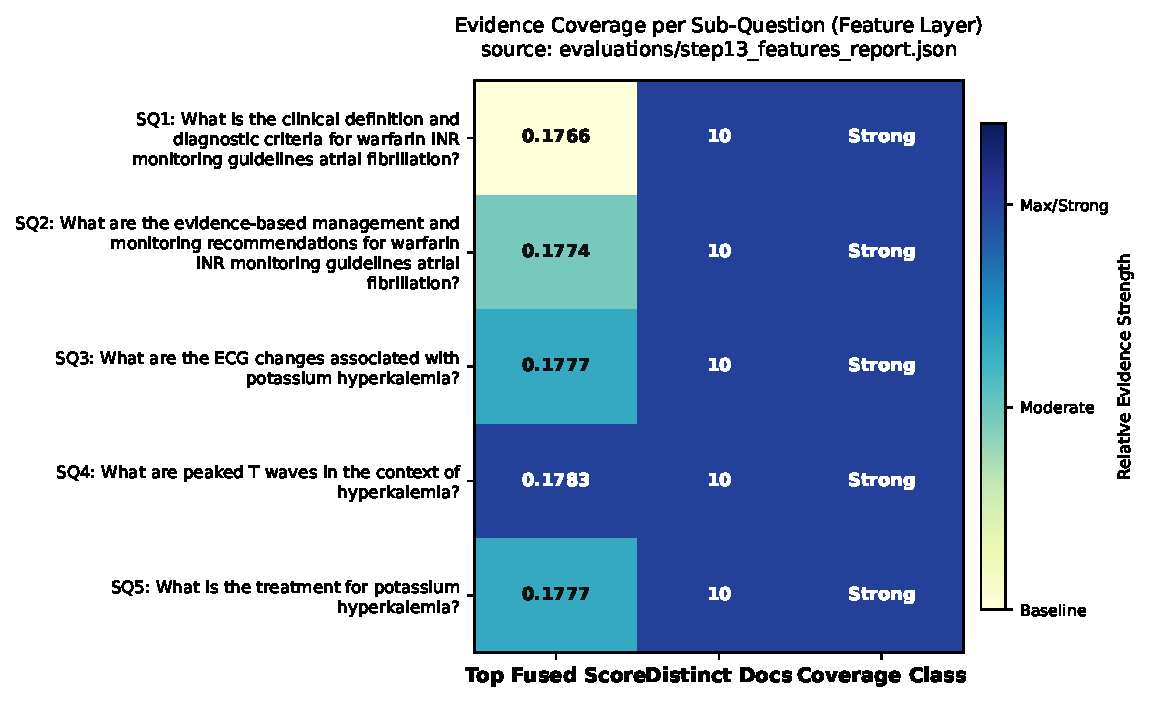
\includegraphics[width=\textwidth]{figures/coverage_heatmap.pdf}
\caption{Sub-question evidence coverage for the two feature-layer queries:
top fused score, distinct document count, and coverage class for each of the
five atomic sub-questions (all classified \texttt{strong}). Source:
evaluation artifact \texttt{step13\_features\_report.json}.}
\label{fig:coverage}
\end{figure*}

\subsection{MedTrend: Longitudinal Laboratory Trajectory}

POST /api/v1/features/trend accepts a patient's lab-value time series,
classifies each biomarker as \emph{worsening}, \emph{improving}, or
\emph{stable}, and computes a rate of change per month. Significance is
flagged when a value crosses a reference threshold. In the Step-13 evaluation:
Creatinine trended from 97.24 to 167.96~$\mu$mol/L ($+22.90$/month, worsening;
crossed upper threshold 115.0); HbA1c from 6.9\% to 7.8\%
($+0.29$/month, worsening). Graph-derived causal candidates
(LabTest(Creatinine) $\rightarrow$ Disease(Chronic Kidney Disease)) are
returned alongside numerical results.

\subsection{CareGap: Guideline Reconciliation}

POST /api/v1/features/caregap maps patient conditions to evidence-based
guidelines and identifies missing or out-of-target checks. In the Step-13
evaluation for a patient with Type~2 Diabetes and Hypertension: HbA1c was
flagged out-of-target at 8.2\% (guideline: $<$7.0\% for most non-pregnant
adults, source: PMC9107726); creatinine, urine albumin, and renal function
checks were flagged as missing per NICE chronic kidney disease
guidelines~\cite{niceguidelines2024, who2023}. All gaps include PMID/NICE
provenance.

\subsection{CoverageMap: Sub-Question Evidence Coverage}

POST /api/v1/features/coverage decomposes a query into sub-questions and
reports retrieval coverage per sub-question. Letting $s$ denote a
sub-question's top fused score and $d$ its distinct document count, we define
coverage classes:

\begin{equation}
\mathrm{class}(q) =
\begin{cases}
\text{strong}  & s \ge 0.12 \wedge d \ge 2 \\
\text{partial} & 0.03 \le s < 0.12 \vee (s \ge 0.12 \wedge d = 1) \\
\text{none}    & s < 0.03 \vee d = 0
\end{cases}
\label{eq:coverage}
\end{equation}
Eq.~(\ref{eq:coverage}) distinguishes well-supported, partially supported, and
unsupported sub-questions, enabling the frontend to offer rephrasing suggestions
only where retrieval is weak.

For \emph{``warfarin INR monitoring guidelines atrial fibrillation''}, both
sub-questions achieved strong coverage (top fused score 0.1774, 10 distinct
documents). For \emph{``potassium hyperkalemia ECG changes peaked T waves
treatment''}, all three sub-questions achieved strong coverage (top fused
scores 0.1777--0.1783, 10 distinct documents each) (Fig.~\ref{fig:coverage}).

% ─── VII. API and Security ───────────────────────────────────────────────────
\section{API and Security Design}

The FastAPI service (v1.0.0) exposes a versioned REST interface under
/api/v1 with JWT bearer token authentication; guest tokens are auto-purged on
logout. Parallel query serialization is enforced by an asyncio lock, confirmed
in the Step-11 proof (Request~A 5{,}541~ms, Request~B 10{,}637~ms, total wall
time 10{,}647~ms). Destination isolation returns HTTP~403 for cross-user store
access (1.10~ms, 117~bytes). The health endpoint responds in $<$2~ms at both
cold and warm states. All 7/7 Step-11 API security criteria passed.

% ─── VIII. Discussion ────────────────────────────────────────────────────────
\section{Discussion}

\noindent\textbf{i) Safety-first trade-off.}\\*
The 82--88\% refusal rate of the full
verified system will appear unfavorable in accuracy-centric leaderboards.
For a clinical information tool operating on a 50-question USMLE sample
without access to the full medical knowledge necessary to answer every
question, refusing is the correct response. The wrong-assertion rate of 12\%
(C1) versus 44\% (unverified baseline, C4) shows that the verification layer is the
primary safety mechanism (Fig.~\ref{fig:disposition}).

\begin{figure}[!htbp]
\centering
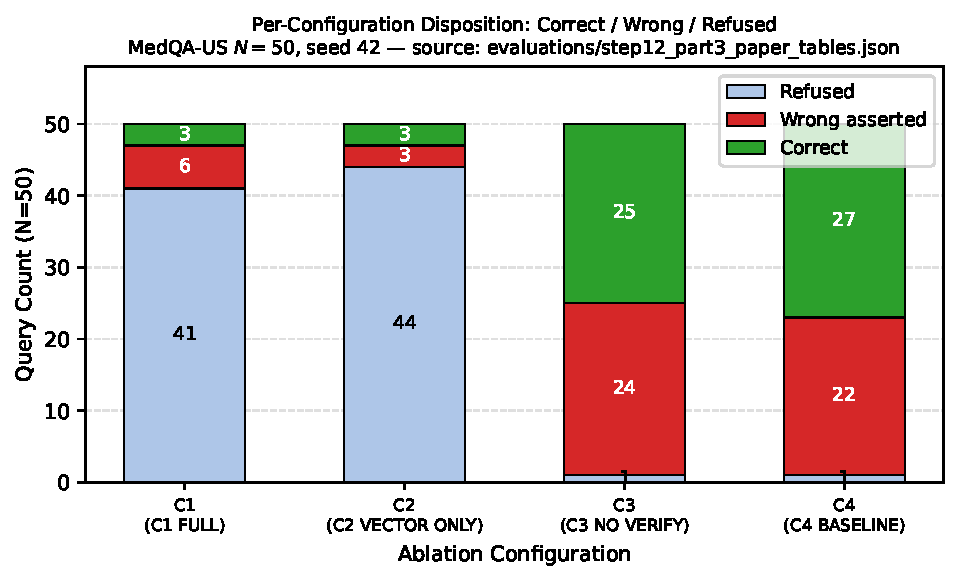
\includegraphics[width=\columnwidth]{figures/disposition_chart.pdf}
\caption{Per-configuration outcome disposition on MedQA-US ($N=50$): counts
of correct, wrong-asserted, and refused queries. Verification shifts outcomes
from wrong assertions toward structured refusals. Source: evaluation artifact
\texttt{step12\_part3\_paper\_tables.json}.}
\label{fig:disposition}
\end{figure}

\noindent\textbf{ii) Graph traversal utility.}\\*
In our ablation, graph traversal did not
improve Accuracy~(All) within verified configurations (both C1 and C2 achieve
6.00\%), but it consistently increased citation richness (9.78 vs.\ 9.18 avg
citations). Graph paths provide interpretable provenance that dense retrieval
cannot: a clinical reviewer can trace an answer to a specific
entity-relationship path, not merely a similarity score.

\noindent\textbf{iii) Limitations.}\\*
The evaluation uses $N=50$ questions, which limits
statistical power. The LLM (Qwen2.5-7B) is not fine-tuned on medical data,
and the high refusal rate partly reflects the model's calibration on general
instruction-following data rather than clinical question answering. Scaling
to $N=500$ and fine-tuned models is a natural extension. The latency of the
full verified system (15{,}386~ms median) is above the 10~s threshold
comfortable for interactive use; graph traversal optimization and batched
verification are future work.

\noindent\textbf{iv) Broader impact.}\\*
MedGraphRAG is designed as a patient-safety system,
not a diagnosis engine. Every response carries a mandatory disclaimer and
never claims diagnostic authority. The AES-256-GCM encrypted private store
ensures patient data confidentiality at rest. All feature-layer evaluations
used synthetic fixture reports; no real patient data was processed.

% ─── IX. Conclusion ──────────────────────────────────────────────────────────
\section{Conclusion}

We presented MedGraphRAG, a self-verifying graph-augmented RAG system for
medical question answering deployable on consumer hardware. Our ablation study
demonstrated that a LangGraph verification agent reduces the clinically
critical wrong-assertion rate from 44\% (unverified baseline, C4) to 12\% (full
system) on MedQA-US ($N=50$). The hybrid FAISS+K\`{u}zu retrieval pipeline
achieves 47.1~ms mean retrieval latency over a 2.29M-vector index. The
complete system operates within 3.62~GB peak RAM and 4{,}784~MB VRAM,
enabling deployment on commodity clinical workstations. Three validated
feature-layer utilities provide longitudinal trend analysis, guideline
reconciliation, and evidence coverage mapping. While current evaluation is
constrained to single-turn benchmarks and serialized single-GPU execution,
future work will expand multi-turn clinician workflows and distributed graph
partitioning. Source code, evaluation scripts, and all JSON evaluation
artifacts will be released publicly upon acceptance.

% ─── References ──────────────────────────────────────────────────────────────
\bibliographystyle{IEEEtran}
\bibliography{references}

\end{document}
